% Copyright © 2015 Martin Ueding <dev@martin-ueding.de>

\documentclass[11pt, english, fleqn, DIV=15, headinclude, BCOR=1cm]{scrartcl}

\usepackage[bibatend, color]{../header}

\usepackage{tikz}

\usepackage[tikz]{mdframed}
\newmdtheoremenv[%
    backgroundcolor=black!5,
    innertopmargin=\topskip,
    splittopskip=\topskip,
]{theorem}{Theorem}[section]

\hypersetup{
    pdftitle=
}

\newcounter{totalpoints}
\newcommand\punkte[1]{#1\addtocounter{totalpoints}{#1}}

\newcounter{problemset}
\setcounter{problemset}{3}

\subject{Geometry in Physics}
\ihead{Geometry in Physics -- Problem Set \arabic{problemset}}

\title{Problem Set \arabic{problemset}}

\publishers{Group 1 -- Jens Boos}
\ofoot{Group 1 -- Jens Boos}

\author{
    Martin Ueding \\ \small{\href{mailto:mu@martin-ueding.de}{mu@martin-ueding.de}}
    \and
    Paul Manz \\ \small{\href{mailto:paul.manz@dreiacht.de}{paul.manz@dreiacht.de}}
}
\ifoot{Martin Ueding, Paul Manz}

\ohead{\rightmark}

\usepackage{multicol}

\renewcommand\thesubsection{\thesection.\alph{subsection}}

\begin{document}

\maketitle

\vspace{3ex}

\begin{center}
    \begin{tabular}{rrr}
        problem number & achieved points & possible points \\
        \midrule
        1 & & \punkte{20} \\
        2 & & \punkte{20} \\
        3 & & \punkte{10} \\
        \midrule
        Total & & \arabic{totalpoints}
    \end{tabular}
\end{center}

\section{Alternating forms}

\subsection{Vector space}

The forms we consider here are still linear by the definition on the problem
set. Since $\phi$ is linear in all of its arguments, the definition of
addition and scalar multiplication is straightforward. Since we consider the
whole space of those alternating forms, the space is also closed under
those operations. It must be a vector space.

\subsection{Small $p$}

In the definition of the space of alternating forms, the number $p$ said
how many elements of $V$ are needed for the from to produce a real value from
the field $\R$. So for $p = 0$, the resulting space is $\Lambda^0(V^*)$
which contains all the forms that do not take any element from $V$ to produce a
scalar. These are all the elements of $\R$ itself.

Now for $p = 1$ one needs to give the 1-form $\phi$ one element from $V$
to get a scalar. Since it only has one argument, it cannot be not
antisymmetric in it. So \emph{any} 1-form is antisymmetric in this sense.
Therefore all of $V^*$ is allowed and we have $\Lambda^1(V^*) = V^*$.

\subsection{Large $p$}

Here we have an $n$-dimensional vector space and consider $p$-forms with $p >
n$ on that. The problem is that there are only $n$ independent vectors in an
$n$-dimensional space. Since it is multilinear the whole thing can be expressed
in terms of the basis vectors $\{\ev_i\}$ of the vector space. The action of
$\phi$ on a set of $p$ vectors can be expanded in terms of basis vectors. We
start with expression the vectors in the basis:
\begin{align*}
    \phi(\vec v_1, \ldots, \vec v_p)
    &= \phi(v_1^i \ev_i, \ldots, v_p^k \ev_k).
    \intertext{%
        Now we can use the linearity in each argument of $\phi$ and pull all
        the scalars out.
    }
    &= v_1^{i} \ldots v_p^k \phi(\ev_i, \ldots, \ev_k).
\end{align*}
The only way a summand in the implied sum can give a non-zero contribution is
that all the indices $i, \ldots, k$ are pairwise different. Since $i, \ldots, k
\in \N \cap [1, n]$, this is not possible! The only \emph{alternating} form
that could be defined is zero.

\subsection{Dimensionality}

The dimensionality of a space is equal to the number of basis vectors. We will
show here that the number of basis vectors of the space of alternating forms is
$\binom np$. We want $p$-forms, they therefore need to take $p$ vectors as
arguments and generate a scalar from them. Since they form a vector space,
every form can be written as a linear combination of basis elements. The forms
are contained in the space $\otimes^p V$. The basis elements of this tensor
space can be
written as
\[
    \bigotimes_{k=0}^p \ev^{i_k}.
\]
where the $\{i_k\}$ are out of $\N \cap [1, n]$ but not necessarily unique at
this point. In other words, one has an $n$-dimensional space where one wants to
create a linear mapping that takes $p$ vectors as arguments. Those multilinear
mappings can be written as products of simple linear mappings. To illustrate
this with $p = 2$ here: Let $\phi(\vec u, \vec v) = \lambda$ be such a bilinear
mapping. Then we can write this as
\[
    \phi(\vec u, \vec v) = u^i v^j \phi(\ev_i, \ev_j).
\]
The $n^2$ components $\phi(\ev_i, \ev_j)$ completely describe the mapping. We
can write $\phi$ in components as
\[
    \phi = \phi_{ij} \ev^i \otimes \ev^j.
\]
Now $\phi$ can be thought of as a (0, 2) tensor which has $n^2$ components. Now
comes the restriction part: Since this tensor has to be completely
antisymmetric in all its indices, there is just one degree of freedom left, the
magnitude of the $\phi_{12}$ component. Therefore, with $n = p = 2$, it
actually is $\binom 22$. To generalize this to $n = 3$ but keeping $p = 2$ the
basis vectors are now the following:
\[
    \ev^1 \otimes \ev^2
    \eqnsep
    \ev^2 \otimes \ev^3
    \eqnsep
    \ev^3 \otimes \ev^1
\]
So there are three basis elements for two-forms in a three dimensional space.
This is because there are $\binom np$ ways of selecting $p$ unique elements of
a set with cardinality $n$. The $\phi_{ij\ldots k}$ does not introduce any more
degrees of freedom as shown above.

\section{Exterior algebra}

\subsection{Maximum order}

\begin{small}
    $n$ is not defined again in this problem, but we will just assume it is the
    dimensionality of $V$ just like before. And the second $\phi$ probably is a
    $\psi$, otherwise it would be defined twice.
\end{small}

$\psi$ already is an alternating form with maximum order on the space $V$.
Adding another order to it (and this is going to happen since $p > 0$) will
make it identical to zero since there is no alternating form with $p > n$ as
shown earlier.

This can also be shown in index notation. we use antisymmetrization notation by
\textcite{penrose-road_to_reality} in the idempotent form which looks like
this:
\[
    \phi_{[ij]k} = \frac{1}{2!} \sbr{ \phi_{ijk} - \phi_{jik} }.
\]
Now Equation~(3) from the problem set becomes:
\begin{align*}
    [\phi \wedge \psi](\vec v_1, \ldots, \vec v_p, \vec v_{p+1}, \ldots, \vec v_{p + n})
    &= \frac{[p + n]!}{p!n!}
    \phi(\vec v_{[1}, \ldots, \vec v_p) \psi(\vec v_{p+1}, \ldots, \vec v_{p+n]}).
    \intertext{%
        The factor $[p+q]!$ is needed by my choice of idempotent
        antisymmetrization. Now we can expand each vector $\vec v_i$ in terms of
        its components and basis vectors and define each form in terms of its
        basis elements as well. This needs the introduction of another set of
        indices to sum over. The antisymmetrization stays at the vector
        components in this step.
    }
    &= \frac{[p + n]!}{p!n!}
    \phi_{i\ldots j} \psi_{k \ldots l}
    \vec v_{[1}^i \ldots \vec v_p^j \vec v_{p+1}^k \ldots \vec v_{p+n]}^l
    \intertext{%
        We can now move the antisymmetrization to the forms $\phi$ and $\psi$.
        Here we have a notational challenge: The indices are now multiple
        symbols, so we could delimit them with commas. But commas in indices
        denote partial derivatives. We will just leave it like this and hope
        the intent is clear.
    }
    &= \frac{[p + n]!}{p!n!}
    \phi_{[1\ldots p} \psi_{p+1\ldots p+n]}
    \vec v_{1}^i \ldots \vec v_p^j \vec v_{p+1}^k \ldots \vec v_{p+n}^l
    \intertext{%
        The expression $\phi_{[1\ldots p} \psi_{p+1\ldots p+n]}$ now denotes a
        completely antisymmetric $p+q$ dimensional form. The problem is that
        this is in an $n$ dimensional vector space which does not work: The
        antisymmetrization will pick up at least one index twice and therefore
        create pairs of terms with opposing signs. Those cancel each other and
        all is left is
    }
    &= 0.
\end{align*}

Once the forms are expressed with indices, the Equation~(3) from the problem
set can be written shorter as:
\[
    [\phi \wedge \psi]_{i\ldots kl \ldots m} = \frac{[p + n]!}{p!n!}
    \phi_{[i\ldots k} \psi_{l \ldots m]}.
\]

\subsection{Bilinearity}

In the above equation, there is a simple product of two quantities, so it has
to be bilinear:
\begin{align*}
    \sbr{[\phi + c \tilde \phi] \wedge \psi}_{i\ldots kl \ldots m}
    &= \frac{[p + n]!}{p!n!}
    [\phi + c \tilde \phi]_{[i\ldots k} \psi_{l \ldots m]}
    \intertext{%
        Since the forms themselves are in a vector space, we can assign the
        indices to each one. The antisymmetrization notation breaks there,
        though. So we then also expand the product and obtain
    }
    &= \frac{[p + n]!}{p!n!}
    \phi_{[i\ldots k} \psi_{l \ldots m]}
    + c \tilde \phi_{[i\ldots k} \psi_{l \ldots m]}.
    \intertext{%
        Now we can pick up the shards and write this more compactly as
    }
    &= \phi \wedge \psi + c \tilde\phi \wedge \psi.
\end{align*}

\subsection{Associativity}

We have just shown the bilinearity by reducing the wedge product to a product
of two simple numbers. For those, the associativity also holds.

\subsection{Graded commutativity}

Look at
\[
    [\phi \wedge \psi]_{i\ldots kl \ldots m} = \frac{[p + n]!}{p!n!}
    \phi_{[i\ldots k} \psi_{l \ldots m]}
\]
again. In order to swap them both, we need to swap the indices $i \ldots k$
with the set $l \ldots m$. For each index of the last set ($q$ of them) we need
to swap them through all the indices of the first set ($p$ of them). Each
swapping will change the sign because the forms are antisymmetric. In total
there are $pq$ swappings needed, therefore the total sign change is
$[-1]^{pq}$.

\section{Directional derivative}

\subsection{Concrete values}

We have
\[
    \vec p(t) =
    \begin{pmatrix}
        \cos(t) \\ \sin(t)
    \end{pmatrix}
    \eqnsep
    \vec v =
    \begin{pmatrix}
        1 \\ 0
    \end{pmatrix}
\]
and the function $f(x, y) = \frac12 [x^2 + y^2]$.

\subsection{Sketches}

The plots of $f$ are shown in Figure~\ref{fig:f}.
Figure~\ref{fig:vector-fields} shows the gradient $\dif f$ and $\vec v = \vec
p(0)$.

\begin{figure}[htbp]
    \centering
    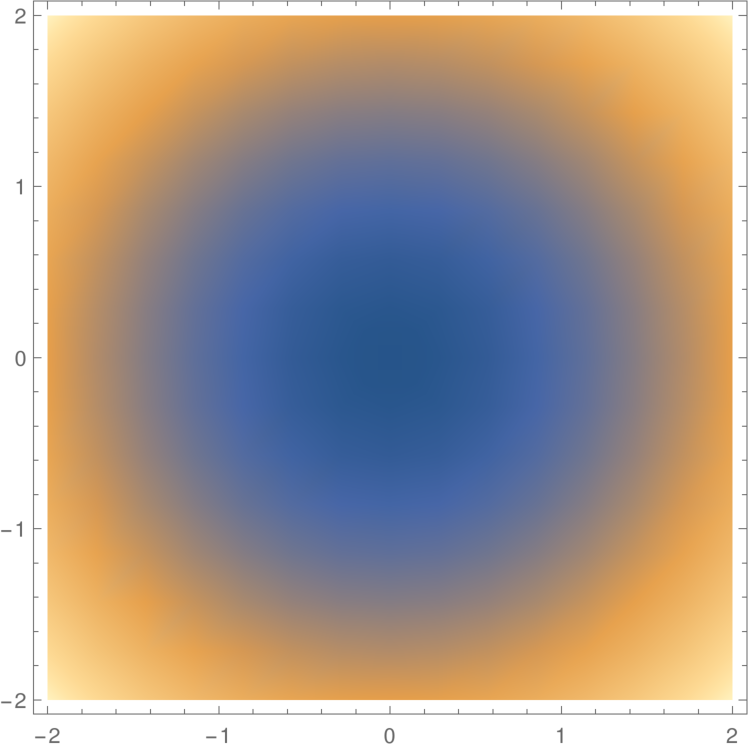
\includegraphics[width=.45\linewidth]{headmap.pdf}
    \hfill
    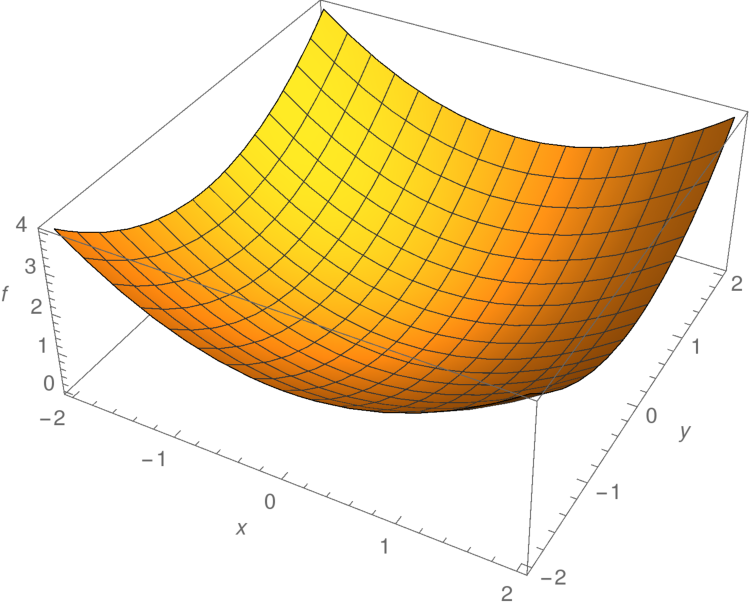
\includegraphics[width=.45\linewidth]{3dplot.pdf}
    \caption{%
        Visualizations of $f(x, y)$. The left one shows a good representation
        of $f$ as a member $C^\infty(\R^2, \R)$ since it the value at each
        point is a scalar and the domain is a two dimensional surface. The
        right side shows a 3D plot of the same function. The problem with this
        visualization is that it suggests that $f$ embedded in $\R^3$ or
        something similarly. It is better to think intrinsically to get beyond
        submanifolds. Created with \emph{Mathematica} 10.
    }
    \label{fig:f}
\end{figure}

\begin{figure}[htbp]
    \centering
    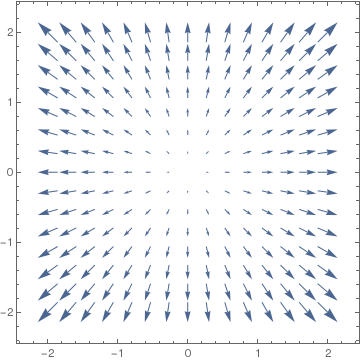
\includegraphics[width=.45\linewidth]{gradient.png}
    \hfill
    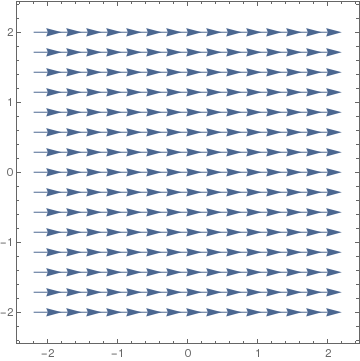
\includegraphics[width=.45\linewidth]{v.png}
    \caption{%
        The left side shows $\vec\partial f$. Either the coordinates are
        $(\ev^1, \ev^2)$ and this is the actual gradient $\dif f$, which is a
        1-form. Or the axes show $(\ev_1, \ev_2)$ and the plot shows 
        the vector field $[\dif f]^\sharp$. Since we are working in $\R^2$,
        there probably is an Euclidean metric and this can be done trivially.
        The right side visualizes $\vec v$, which is an actual vector. It is a
        rather boring vector field since it is constant everywhere. $\vec p(t)$
        looks just the same, except that it is rotated by the angle $t$ (in
        radians, of course).
        Sorry for the rastered images, \emph{Mathematica 10} had some problem
        exporting those as PDF or EPS files.
    }
    \label{fig:vector-fields}
\end{figure}

\end{document}

% vim: spell spelllang=en tw=79
